\section{Components and high level requirements}
\label{sec:high_level_requirements}

From the challenges in creating hybrid board games, we believe that an platform for creating augmented boardgames can all involved roles greatly. The role of a game designer requires knowledge of game concepts, and has a great challenge of creating an entertaining game and balancing randomness with skill and knowledge. A game designer could be assisted by helping the creative process or simplify the concepts that a board game can consist of. A game designer has technical challenges, and the lack of existing, suitable hardware tokens and tools for integrating them with a user friendly mobile surface can make the implementation of the game very time consuming. From testing Don't Panic, we know that acquisition of hardware tokens should be cheap, and games easier to set up. Tokens should also preferably be reusable to other games for people without technical knowledge. We also think that the marked for such games is too small to be easily discoverable.

\subsection{High level requirements}

We have chosen to focus mainly on the challenges of the developer, and assist him or her in the implementation process of hybrid board games.

\begin{itemize}
\item D1 - A \textbf{game developer} should be able to extend or remove parts of the AnyBoard platform, in order to suit his or her needs that are not originally covered by the platform.
\item D2 - A game developer should not be required to pay for creating games through the AnyBoard platform, in order to lower the barrier for using AnyBoard.
\item D3 - A game developer should not be required to rewrite his or her game in order to be supported on different platforms or screen sizes, so to minimize the development effort necessary to reach a broad audience.
\item D4 - A game developer should be assisted with guidance on how to compile and deploy the applications to Google Play (Android) and App Store (iOS), in order to simplify the development and distribution of games made with AnyBoard.
\item D5 - A game developer should be provided with an API for communicating with supported digital tokens, and not be required knowledge of low-level code, in order to lower the barrier for using the AnyBoard platform.
\item D6 - A game developer should be able to extend digital token support to new tokens with new features with example code and written guides, in order not to restrict the developer to a fixed set of tangible tokens.
\item D7 - A game developer should be provided with classes and abstractions for typical board game entities, such as boards, pawns, dices, cards and decks, in order to lower the development time.
\item D8 - A game developer should be provided with a basic set of visual elements for screen display, such as menus, cards, boards, pawns, timers and buttons, in order to lower the development time.
\item D9 - A game developer should be provided with signals and event handlers to simplify implementing responses to a players actions, and game events.
\end{itemize}
\begin{itemize}
\item P1 - \textbf{A player} should not be required to have technical competence in order to initialize a game made with AnyBoard, in order to lower the barrier for players to acquire an augmented board game.
\item P2 - A player should be able to reuse board game hardware to play other games with ease, in order to lower the barrier for players to try other hybrid board games once having acquired one.
\end{itemize}

\subsection{Main components}
We present here a broad idea for how we can fulfill these requirements and create tools to accomodate and help developers and players to create and use hybrid board games. A sketch of this can be seen in figure \ref{fig:high_level_components}.

\begin{figure}[ht]
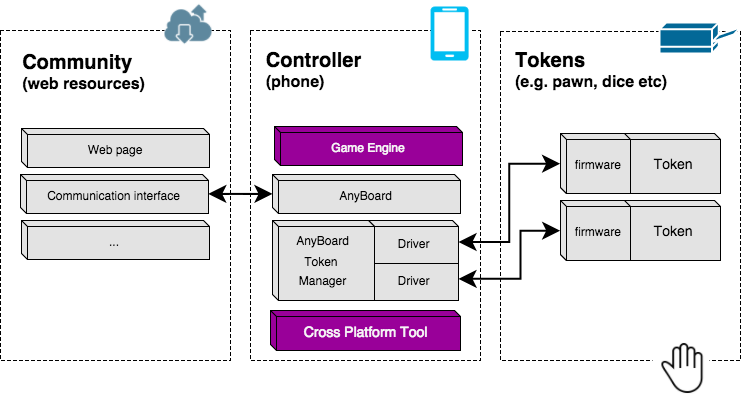
\includegraphics[width=12cm]{img/broad_architecture_idea.png}
\centering
\caption{High level components of AnyBoard.}
\label{fig:high_level_components}
\end{figure}

Game development tools and communities already exists, and hence the main part that makes the AnyBoard platform unique, is helping integrate the tangible tokens as a part of games. This is therefore the area of greatest importance. 

\emph{Standard example tokens}, with low level code implementing typical token capabilities, will be provided for developers that wish to create games with general token requirements. This token will communicate with a \emph{Token manager} on the application side that handles the communication between the game logic and physical devices. This component will provide a token API on the software side, so developers can listen to token-events and send commands without the knowledge of the low level code, as well as assist developers to create easy-to-use interfaces for connecting and initiating the game and game tokens.  \emph{(P1, D5)}

The Token manager is separated from any spesific token, and communicates through a \emph{device spesific driver}. A generic extendable driver will be provided to assist developers that wish to create their own tokens with other capabilities. \emph{(D1, D6)}

A \emph{Game engine} will provide tools that help the developer quickly create the components of his or her game. We wish to provide base components spesificly suited for hybrid board games, such as Board, Tile, Pawn, Dice etc, both the logical and visual \emph{UI} part. \emph{(D7, D8, D9)}

The AnyBoard software platform should be based on a \emph{cross platform tool} that enable games made with the AnyBoard to compile to different operating systems. \emph{(D3, D4)}

Several of these components exists already, and we aim to use open source, free-to-use, modular and well documented tools, so that a developer can pick apart the AnyBoard system and add capabilities where need be. \emph{(D1, D2)}

Lastly, a web-based home for AnyBoard can grow a community and provide information for all roles involved with hybrid board games. The AnyBoard platform could be downloaded from here, and tokens sold from a web store. It can also provide a knowledge base and tools for developers to assist each other. Through a \emph{Game Store} or an overview of hybrid board games, we hope to assist users with finding other games they can play, and an assistive IDE for game developers could help lower the knowledge barrier for new developers even further. \emph{(P2)}\footnote{A game store, or a web based IDE is a later stage than the AnyBoard platform presented in this thesis.}. 



